% ==================== CHƯƠNG 1 ====================
\chapter{KHẢO SÁT BÀI TOÁN}
\section{Mô tả yêu cầu bài toán}
Mục tiêu của bài toán là phát triển một hệ thống website hỗ trợ tổ chức, quản lý và theo dõi các lớp học thêm và nhóm gia sư tư thục với các tính năng chính bao gồm: quản lý người dùng và phân quyền (Gia sư/Giáo viên, Học sinh, Phụ huynh); quản lý lớp học, lịch học và danh sách học sinh; điểm danh; quản lý bài tập, bài kiểm tra và cập nhật điểm số; quản lý học phí; cung cấp thông tin minh bạch để học sinh và phụ huynh theo dõi tiến độ học tập.

Hệ thống cho gia sư/giáo viên có thể tạo và quản lý lớp học, lập thời khóa biểu, thực hiện điểm danh, cũng như nhập và cập nhật điểm số, bài tập, bài kiểm tra cho học sinh. Học sinh có thể xem lịch học, điểm số, kết quả và thông tin của bản thân để dễ dàng theo dõi quá trình tiến bộ. Phụ huynh có thể theo dõi sát sao tình hình học tập, điểm danh, kết quả và tình trạng học phí của con em mình dựa trên các thông tin do gia sư cập nhật trên hệ thống.

\section{Khảo sát bài toán}
Để phân tích và xây dựng hệ thống quản lý lớp học thêm, nhóm tiến hành khảo sát yêu cầu nghiệp vụ thông qua việc tham khảo các biểu mẫu. Đối tượng khảo sát: Giáo viên/gia sư, phụ huynh và học sinh.

Qua quá trình khảo sát, khó khăn của gia sư/giáo viên cũng như nhu cầu của phụ huynh và học sinh được cụ thể hóa như sau:
\begin{itemize}
    \item \textbf{Đối đối với giáo viên/gia sư:}
    \begin{itemize}
        \item Khó khăn khi quản lý sĩ số và điểm danh bằng sổ tay/Excel (dễ nhầm lẫn, mất thời gian thông báo riêng cho từng phụ huynh).
        \item Quy trình chấm bài, nhập điểm và gửi kết quả thủ công qua Zalo/Messenger khiến dữ liệu bị phân tán, mất nhiều công sức.
        \item Vất vả trong việc tổng hợp số buổi học, tính toán học phí và theo dõi công nợ thủ công.
    \end{itemize}

    \item \textbf{Đối với học sinh và phụ huynh:}
    \begin{itemize}
        \item {Thông tin muốn theo dõi:} Lịch học, tình hình chuyên cần (điểm danh hằng buổi), điểm số các bài kiểm tra/bài tập, và trạng thái học phí (đã đóng, còn thiếu).
        \item {Hình thức nhận thông báo mong muốn:} Mong muốn có một hệ thống/cổng thông tin tập trung để có thể tra cứu chủ động bất cứ lúc nào thay vì chờ giáo viên nhắn tin hoặc xem tin nhắn bị trôi trên Zalo.
    \end{itemize}
\end{itemize}

Trên cơ sở đó, nhóm đã mô tả quy trình As-Is cũng như đề xuất quy trình To-Be cho các quy trình sau:
%========== QUY TRÌNH ĐIỂM DANH ========
\subsection{Quy trình điểm danh}
%========== AS-IS QUY TRÌNH ĐIỂM DANH ========
\subsubsection{Quy trình hiện tại (As-Is)}
Hiện tại, theo dữ liệu khảo sát, giáo viên quản lý lớp học thêm thực hiện việc điểm danh chủ yếu bằng phương pháp thủ công. Giáo viên sử dụng sổ tay cá nhân hoặc file Excel để ghi nhận sỉ số. Khi phụ huynh có nhu cầu kiểm tra hoặc khi học sinh vắng mặt, giáo viên phải chủ động nhắn tin thông báo qua các ứng dụng như Zalo, Messenger hoặc SMS.
\begin{figure}[htbp]
    \centering
    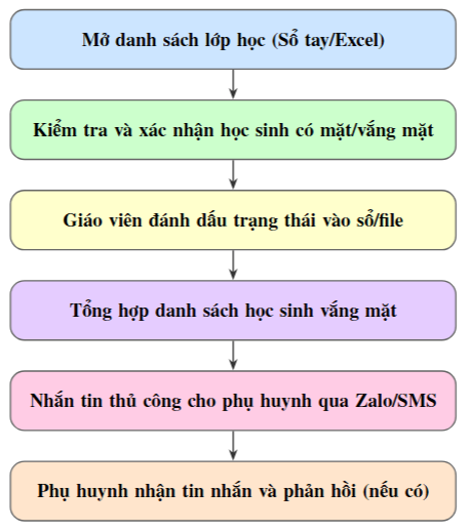
\includegraphics[width=0.5\textwidth]{picC1/diem-danh-as-is.png}
    \caption{Sơ đồ quy trình điểm danh As-Is}
\end{figure}

\noindent \textbf{Mô tả chi tiết quy trình As-Is:}
\begin{itemize}
    \item \textbf{Bước 1 – Mở danh sách lớp:} Khi bắt đầu buổi học, giáo viên mở sổ điểm danh giấy hoặc file Excel đã chuẩn bị sẵn.
    \item \textbf{Bước 2 – Kiểm tra sĩ số:} Giáo viên gọi tên hoặc quan sát lớp để xác định những học sinh có mặt, đi trễ hoặc vắng mặt.
    \item \textbf{Bước 3 – Đánh dấu trạng thái:} Giáo viên ghi chép trạng thái chuyên cần của từng học sinh vào sổ hoặc nhập vào file Excel.
    \item \textbf{Bước 4 – Tổng hợp vắng mặt:} Cuối buổi học hoặc ngay lúc đó, giáo viên lọc ra danh sách các em không tham gia buổi học.
    \item \textbf{Bước 5 – Thông báo cho phụ huynh:} Giáo viên mở ứng dụng chat (như Zalo), tìm đúng tên phụ huynh của học sinh vắng mặt và nhắn tin thông báo.
     \item \textbf{Bước 6 – Phụ huynh phản hồi:} Phụ huynh đọc tin nhắn và có thể nhắn lại để xin phép hoặc trao đổi thêm.
\end{itemize}

\noindent \textbf {Các vấn đề của quy trình hiện tại}

Dựa trên kết quả khảo sát, quy trình điểm danh thủ công đang gặp các khó khăn sau:
\begin{table}[htbp]
    \centering
    \caption{Phân tích vấn đề quy trình điểm danh As-Is}
    \renewcommand{\arraystretch}{1.5}
    \begin{tabular}{|c|p{5cm}|p{6.5cm}|}
        \hline
        \textbf{STT} & \textbf{Vấn đề} & \textbf{Ảnh hưởng} \\ \hline
        1 & Ghi nhận điểm danh thủ công trên sổ hoặc Excel. & Mất thời gian, dễ quên lưu lại hoặc đánh dấu nhầm trạng thái của học sinh. \\ \hline
        2 & Việc thông báo vắng mặt qua tin nhắn cá nhân (Zalo, SMS). & Giáo viên tốn thời gian tìm danh bạ, soạn tin nhắn riêng; dễ gửi nhầm người. \\ \hline
        3 & Dữ liệu chuyên cần bị phân tán. & Khó khăn khi cần thống kê số buổi học cuối tháng để tính học phí. \\ \hline
        4 & Phụ huynh thụ động trong việc theo dõi. & Phụ huynh không biết tình trạng đi học của con trừ khi giáo viên chủ động nhắn tin. \\ \hline
    \end{tabular}
\end{table}
%========== TO-BE QUY TRÌNH ĐIỂM DANH ========
\subsubsection{Quy trình đề xuất (To-Be)}
\begin{figure}[htbp]
    \centering
    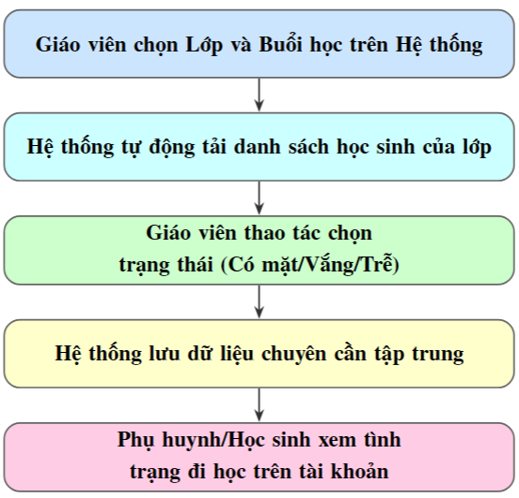
\includegraphics[width=0.5\textwidth]{picC1/diem-danh-to-be.png}
    \caption{Sơ đồ quy trình điểm danh To-Be}
\end{figure}

\noindent \textbf{Mô tả chi tiết quy trình To-Be:}
\begin{itemize}
    \item \textbf{Bước 1 – Chọn lớp và buổi học:} Giáo viên truy cập vào ứng dụng Web, chọn đúng lớp và buổi học hiện tại.
    \item \textbf{Bước 2 – Tải danh sách:} Hệ thống tự động truy xuất cơ sở dữ liệu và hiển thị danh sách học sinh thuộc lớp đó.
    \item \textbf{Bước 3 – Cập nhật trạng thái:} Giáo viên thực hiện thao tác nhấp chuột hoặc chạm để thay đổi trạng thái (Ví dụ: mặc định là "Có mặt", chỉ cần chuyển sang "Vắng" hoặc "Trễ" cho những em tương ứng).
    \item \textbf{Bước 4 – Lưu hệ thống:} Dữ liệu được lưu trữ ngay lập tức vào cơ sở dữ liệu, đảm bảo không bị thất lạc.
    \item \textbf{Bước 5 – Phụ huynh/Học sinh tra cứu:} Phụ huynh và học sinh có thể đăng nhập vào hệ thống bất cứ lúc nào để xem lịch sử chuyên cần một cách minh bạch mà không cần chờ giáo viên nhắn tin.
\end{itemize}

\noindent \textbf {Yêu cầu hệ thống}
\begin{table}[htbp]
    \centering
    \caption{Yêu cầu hệ thống cho quy trình Điểm danh}
    \renewcommand{\arraystretch}{1.5}
    \begin{tabular}{|p{8cm}|c|}
        \hline
        \textbf{Yêu cầu hệ thống} & \textbf{Đối tượng} \\ \hline
        Hệ thống cho phép chọn lớp và hiển thị danh sách học sinh theo buổi học & Giáo viên \\ \hline
        Hệ thống cho phép cập nhật trạng thái điểm danh (Có mặt, Vắng, Trễ) & Giáo viên \\ \hline
        Hệ thống tự động lưu trữ và thống kê số buổi đã học/vắng mặt & Hệ thống \\ \hline
        Hệ thống cho phép phụ huynh xin vắng & Học sinh, Phụ huynh \\ \hline
        Hệ thống tự động lưu trữ và thống kê số buổi đã học/vắng mặt & Hệ thống \\ \hline
        Hệ thống cho phép tra cứu lịch sử điểm danh theo từng học sinh & Học sinh, Phụ huynh \\ \hline
    \end{tabular}
\end{table}

\clearpage
%========== QUY TRÌNH NHẬP VÀ TRẢ KẾT QUẢ HỌC TẬP ========
\subsection{Quy trình nhập và trả kết quả học tập}
%========== AS-IS QUY TRÌNH NHẬP/TRẢ KQ ==========
\subsubsection{Quy trình hiện tại (As-Is)}
Dữ liệu khảo sát cho thấy quy trình quản lý điểm số và kết quả bài tập hiện nay đang bị phân mảnh. Giáo viên chấm bài trên giấy, sau đó nhập điểm vào file Excel cá nhân để lưu trữ. Để thông báo điểm cho học sinh và phụ huynh, giáo viên phải chụp ảnh bảng điểm hoặc nhắn tin riêng lẻ kết quả qua mạng xã hội (Zalo). Quá trình này tốn nhiều công sức và không tạo được một hồ sơ theo dõi sự tiến bộ dài hạn.
\begin{figure}[htbp]
    \centering
    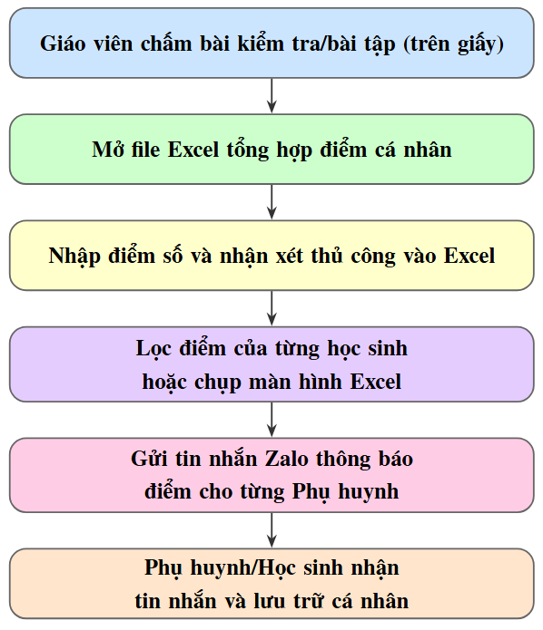
\includegraphics[width=0.5\textwidth]{picC1/nhap-tra-kq-as-is.png}
    \caption{Sơ đồ quy trình nhập và trả kết quả học tập As-Is}
\end{figure}

\noindent \textbf{Mô tả chi tiết quy trình As-Is:}
\begin{itemize}
    \item \textbf{Bước 1 – Chấm bài:} Giáo viên chấm điểm bài kiểm tra, bài tập về nhà của học sinh.
    \item \textbf{Bước 2 – Mở file Excel:} Giáo viên tìm và mở đúng file Excel quản lý điểm của lớp tương ứng.
    \item \textbf{Bước 3 – Nhập điểm:} Giáo viên tiến hành gõ điểm số, đôi khi kèm theo nhận xét ngắn cho từng học sinh vào các cột trong Excel.
    \item \textbf{Bước 4 – Lọc dữ liệu:} Để đảm bảo tính riêng tư, giáo viên không gửi nguyên bảng điểm cho cả nhóm mà phải cắt/ghép hoặc gõ lại điểm của từng em.
    \item \textbf{Bước 5 – Gửi kết quả:} Sử dụng Zalo/Messenger nhắn tin thủ công cho từng phụ huynh/học sinh.
    \item \textbf{Bước 6 – Nhận kết quả:} Phụ huynh đọc tin nhắn. Lịch sử điểm số bị trôi đi theo thời gian giữa các tin nhắn trao đổi khác.
\end{itemize}
\noindent \textbf {Các vấn đề của quy trình hiện tại}

Qua phân tích quá trình thực tế, có thể rút ra các vấn đề nghiêm trọng như sau:
\begin{table}[htbp]
    \centering
    \caption{Phân tích vấn đề quy trình nhập và trả kết quả As-Is}
    \renewcommand{\arraystretch}{1.5}
    \begin{tabular}{|c|p{5cm}|p{6.5cm}|}
        \hline
        \textbf{STT} & \textbf{Vấn đề} & \textbf{Ảnh hưởng} \\ \hline
        1 & Thông báo điểm thủ công qua mạng xã hội (Zalo). & Mất nhiều thời gian, nguy cơ gửi nhầm điểm của học sinh này cho phụ huynh khác. \\ \hline
        2 & Dữ liệu học tập nằm rải rác trên file Excel và tin nhắn. & Không có báo cáo tổng quan về sự tiến bộ của học sinh qua từng tháng. \\ \hline
        3 & Phụ huynh khó theo dõi lịch sử học tập. & Tin nhắn bị trôi, phụ huynh không nhớ điểm bài kiểm tra cũ. \\ \hline
        4 & Thiếu tính liên kết dữ liệu. & Nhập điểm và nhận xét không được kết nối đồng bộ vào hồ sơ chung. \\ \hline
    \end{tabular}
\end{table}
%========== TO-BE QUY TRÌNH NHẬP/ TRẢ KQ =========
\subsubsection{Quy trình đề xuất (To-Be)}
\begin{figure}[htbp]
    \centering
    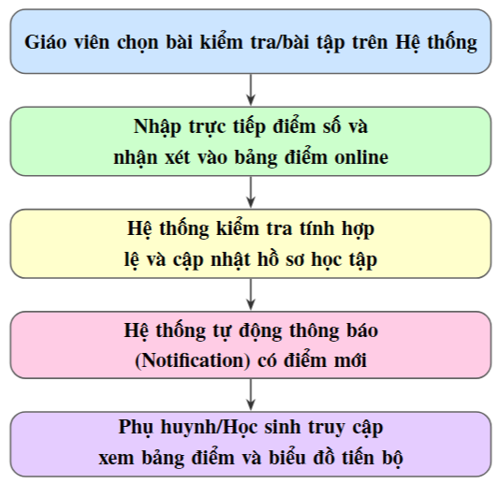
\includegraphics[width=0.5\textwidth]{picC1/nhap-tra-kq-to-be.png}
    \caption{Sơ đồ quy trình nhập và trả kết quả học tập To-Be}
\end{figure}

\noindent \textbf{Mô tả chi tiết quy trình To-Be:}
\begin{itemize}
    \item \textbf{Bước 1 – Chọn bài kiểm tra:} Trên Web Application, giáo viên vào mục Quản lý điểm, chọn lớp và cột điểm cần nhập (ví dụ: Kiểm tra 15p, Bài tập về nhà).
    \item \textbf{Bước 2 – Nhập kết quả:} Hệ thống hiển thị sẵn danh sách lớp, giáo viên chỉ cần điền số liệu vào ô trống và ghi chú nhận xét nếu cần.
    \item \textbf{Bước 3 – Xử lý dữ liệu:} Hệ thống tự động ghi nhận, liên kết điểm số này vào hồ sơ học sinh và có thể tính toán điểm trung bình (nếu được thiết lập).
    \item \textbf{Bước 4 – Thông báo tự động:} Hệ thống gửi thông báo (có thể qua email hoặc notification trên ứng dụng) cho phụ huynh/học sinh.
    \item \textbf{Bước 5 – Minh bạch thông tin:} Phụ huynh đăng nhập vào hệ thống để xem ngay điểm mới, đồng thời có thể xem lại toàn bộ điểm cũ và nhận xét của giáo viên trong suốt quá trình học.
\end{itemize}

\noindent \textbf {Yêu cầu hệ thống}
\begin{table}[htbp]
    \centering
    \caption{Yêu cầu hệ thống cho quy trình Nhập/Trả kết quả}
    \renewcommand{\arraystretch}{1.5}
    \begin{tabular}{|p{8cm}|c|}
        \hline
        \textbf{Yêu cầu hệ thống} & \textbf{Đối tượng} \\ \hline
        Hệ thống cho phép tạo các đầu điểm (Bài tập, Kiểm tra 15p, Giữa kỳ) & Giáo viên \\ \hline
        Hệ thống cho phép nhập điểm và nhận xét trực tiếp cho từng học sinh & Giáo viên \\ \hline
        Hệ thống lưu trữ lịch sử điểm số và tính toán quá trình học tập & Hệ thống \\ \hline
        Hệ thống cho phép xem chi tiết bảng điểm, lịch sử và nhận xét & Học sinh, Phụ huynh \\ \hline
    \end{tabular}
\end{table}

\clearpage
%======== QUY TRÌNH THU HỌC PHÍ ========
\subsection{Quy trình thu học phí}
%======== AI-IS THU HỌC PHÍ ========
\subsubsection{Quy trình hiện tại (As-Is)}
Hiện tại, gia sư/giáo viên thực hiện việc quản lý và thu học phí chủ yếu bằng phương pháp thủ công. Giáo viên phải tự kiểm tra danh sách học sinh, kiểm tra số buổi học, tính số tiền phải thu, thông báo cho phụ huynh và ghi nhận tình trạng thanh toán.
\begin{figure}[htbp]
    \centering
    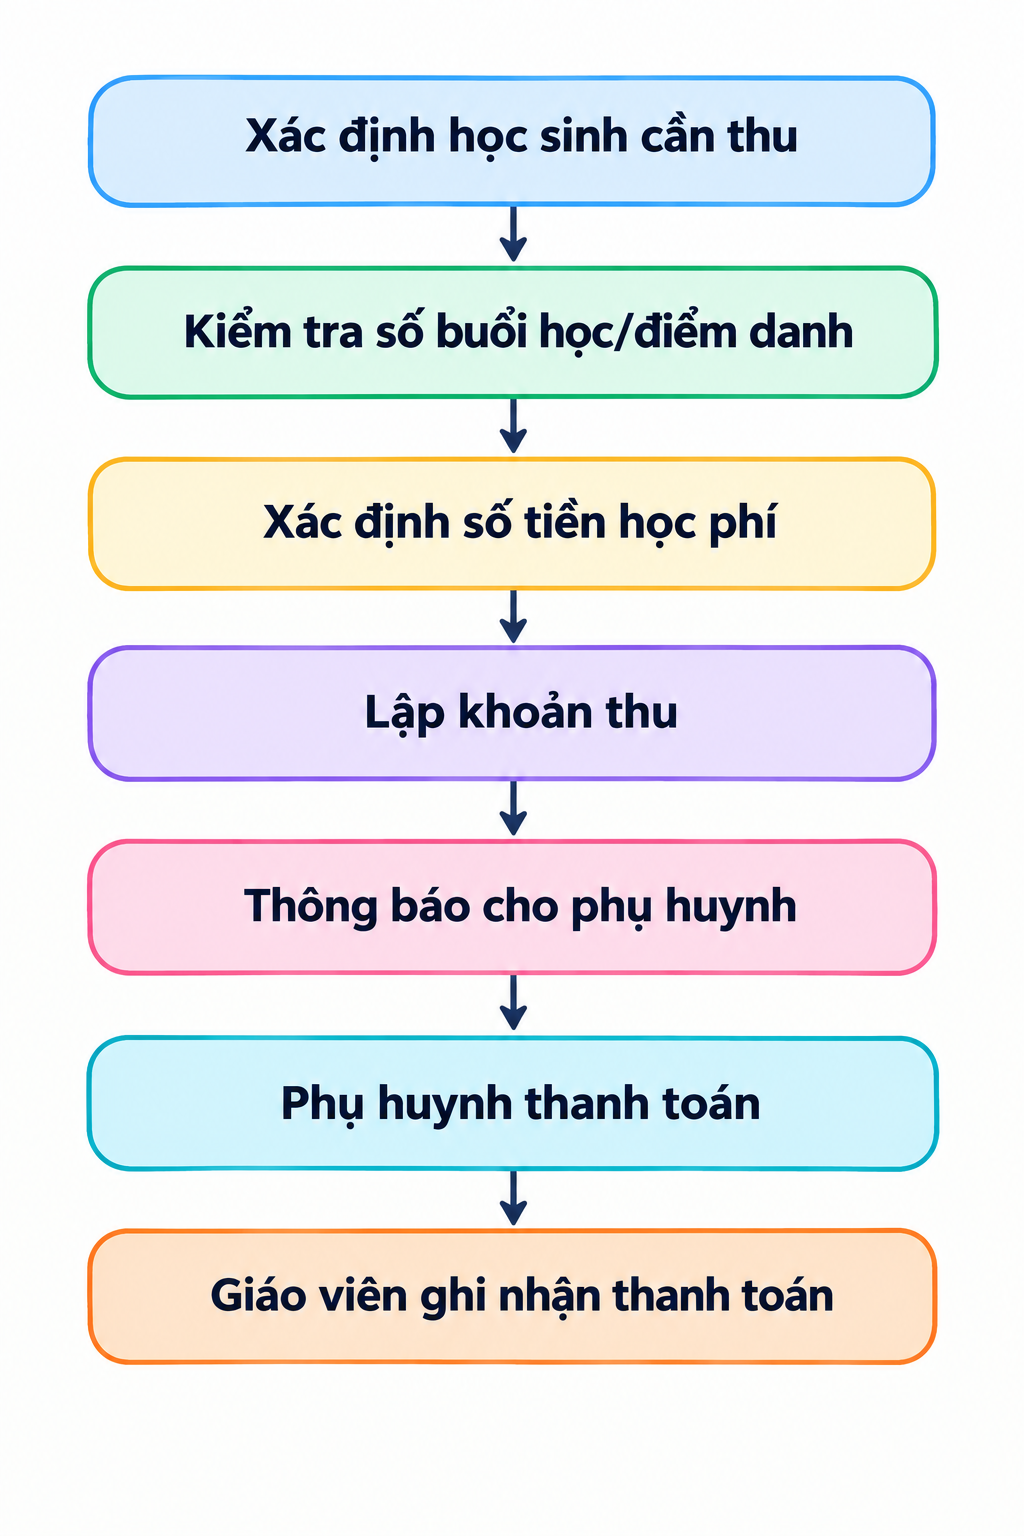
\includegraphics[width=0.5\textwidth]{picC1/thu-hoc-phi-as-is.png}
    \caption{Sơ đồ quy trình thu học phí As-Is}
\end{figure}

\noindent \textbf{Mô tả chi tiết quy trình As-Is:}
\begin{itemize}
    \item \textbf{Bước 1 – Xác định học sinh cần thu:} Gia sư/giáo viên kiểm tra danh sách học sinh để xác định những học sinh đã đến kỳ hoặc tháng cần đóng học phí.
    \item \textbf{Bước 2 – Kiểm tra số buổi học:} Giáo viên kiểm tra dữ liệu điểm danh để xác định số buổi học của từng học sinh trong kỳ/tháng. Việc kiểm tra có thể được thực hiện bằng sổ tay, Excel/Google Sheets hoặc các công cụ quản lý đang sử dụng.
    \item \textbf{Bước 3 – Xác định số tiền học phí:} Dựa trên số buổi học hoặc mức học phí cố định theo kỳ/tháng, gia sư/giáo viên tự tính số tiền học sinh cần đóng.
    \item \textbf{Bước 4 – Lập khoản thu:} Sau khi xác định số tiền, giáo viên ghi nhận thông tin khoản thu bằng sổ tay, file Excel hoặc hình thức quản lý cá nhân khác.
    \item \textbf{Bước 5 – Thông báo cho phụ huynh:} Gia sư/giáo viên thông báo số tiền học phí cần đóng cho phụ huynh thông qua tin nhắn, Zalo, sổ liên lạc hoặc thông qua học sinh.
    \item \textbf{Bước 6 – Phụ huynh thanh toán:} Phụ huynh thực hiện thanh toán cho gia sư/giáo viên bằng tiền mặt hoặc chuyển khoản ngân hàng.
    \item \textbf{Bước 7 – Ghi nhận thanh toán:} Sau khi nhận được tiền, gia sư/giáo viên tự ghi nhận số tiền đã thanh toán vào sổ hoặc file Excel.
    \item \textbf{Bước 8 – Theo dõi số tiền còn thiếu và công nợ:} Trong trường hợp phụ huynh chưa thanh toán hoặc chỉ thanh toán một phần, giáo viên phải tự tính số tiền còn thiếu và tiếp tục theo dõi khoản công nợ.
\end{itemize}

\noindent \textbf {Các vấn đề của quy trình hiện tại}
\begin{table}[htbp]
    \centering
    \caption{Phân tích vấn đề quy trình thu học phí As-Is}
    \renewcommand{\arraystretch}{1.5}
    \begin{tabular}{|c|p{5cm}|p{6.5cm}|}
        \hline
        \textbf{STT} & \textbf{Vấn đề} & \textbf{Ảnh hưởng} \\ \hline
        1 & Kiểm tra điểm danh và tính học phí thủ công. & Tốn thời gian, dễ nhầm số buổi hoặc số tiền phải thu. \\ \hline
        2 & Lưu trữ khoản thu trên sổ, Excel hoặc tin nhắn. & Dữ liệu bị phân tán, khó tra cứu và quản lý tập trung. \\ \hline
        3 & Phụ huynh khó theo dõi thông tin học phí. & Khó biết số tiền phải đóng, đã đóng bao nhiêu và còn thiếu bao nhiêu. \\ \hline
        4 & Ghi nhận thanh toán phụ thuộc hoàn toàn vào giáo viên. & Nguy cơ quên ghi nhận, cập nhật chậm hoặc nhầm lẫn. \\ \hline
        5 & Tổng hợp công nợ thủ công nhiều học sinh. & Dễ bỏ sót hoặc tính sai số tiền công nợ còn lại. \\ \hline
    \end{tabular}
\end{table}

%======== TO-BE THU HỌC PHÍ ========
\subsubsection{Quy trình đề xuất (To-Be)}

\begin{figure}[H] % Dùng [H] viết hoa để ép buộc ảnh nằm đúng vị trí này
    \centering
    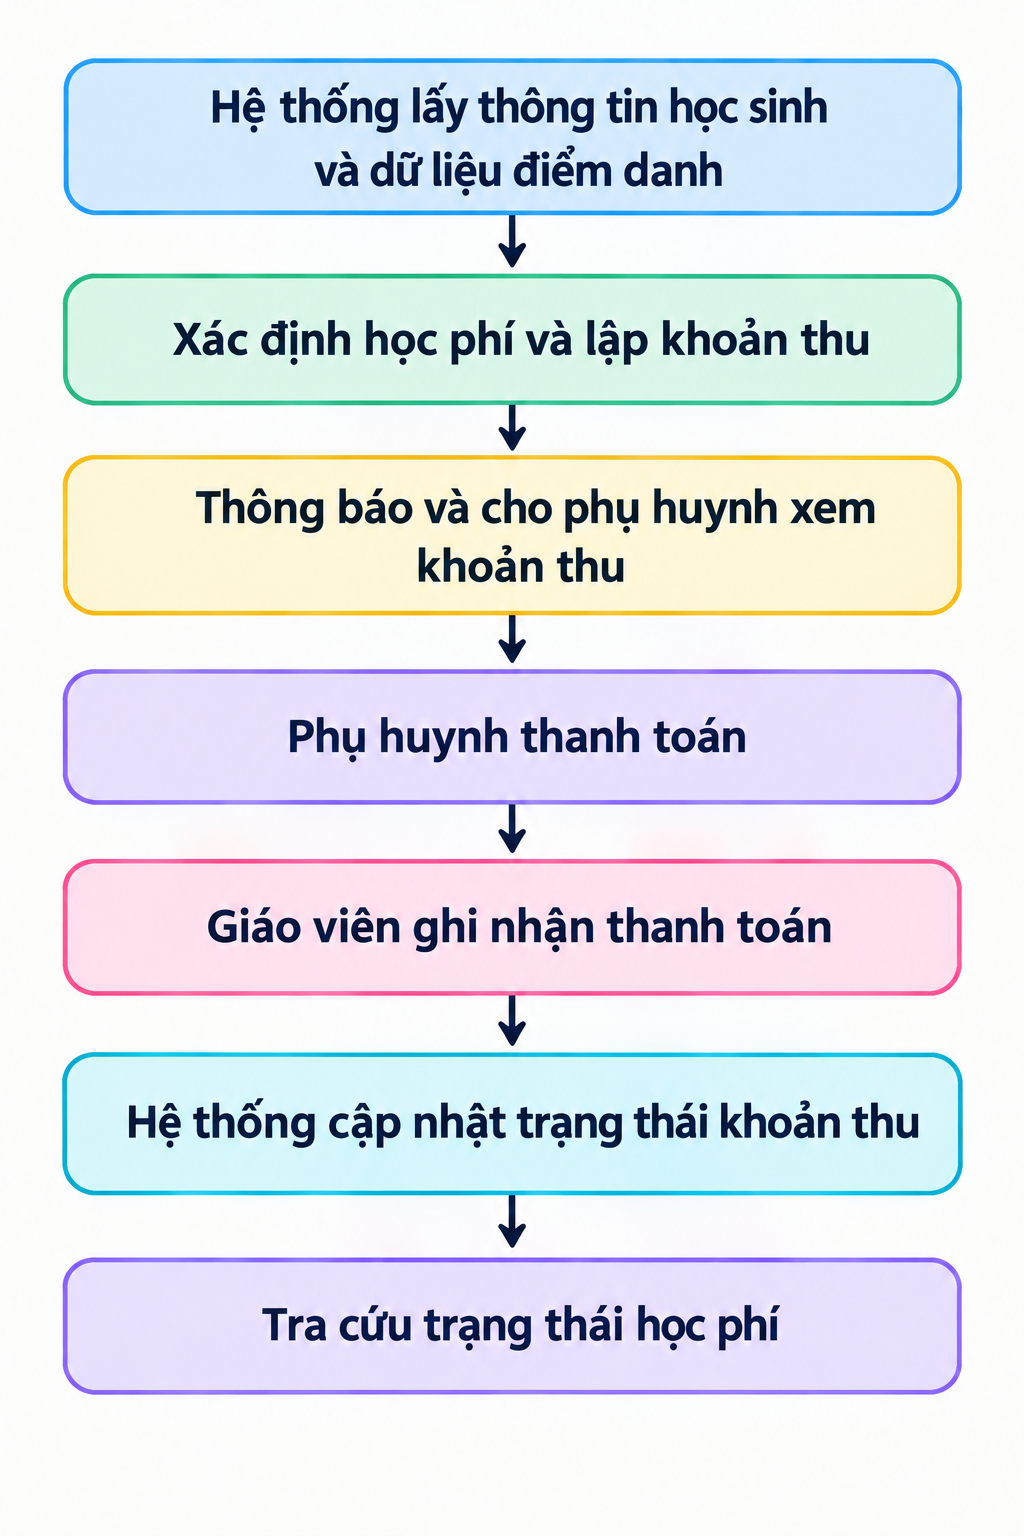
\includegraphics[width=0.5\textwidth]{picC1/thu-hoc-phi-to-be.png}
    \caption{Sơ đồ quy trình thu học phí To-Be}
\end{figure}

\noindent \textbf{Mô tả chi tiết quy trình To-Be:}
\begin{itemize}
    \item \textbf{Bước 1 – Hệ thống lấy thông tin học sinh và dữ liệu điểm danh:} 
    Hệ thống sử dụng thông tin học sinh và dữ liệu điểm danh đã được lưu trong hệ thống để xác định số buổi học của học sinh trong tháng hoặc kỳ tương ứng. Việc sử dụng dữ liệu điểm danh đã có giúp giảm thao tác kiểm tra và đếm thủ công của giáo viên.
    
    \item \textbf{Bước 2 – Xác định học phí và lập khoản thu:} 
    Gia sư/giáo viên kiểm tra thông tin học phí dựa trên dữ liệu của học sinh và thực hiện chức năng “Lập khoản thu” trên hệ thống. Mỗi khoản thu được gắn với học sinh tương ứng và lưu các thông tin cần thiết như:
    \begin{itemize}
        \item Học sinh;
        \item Kỳ/tháng;
        \item Số tiền phải đóng;
        \item Ngày tạo khoản thu.
    \end{itemize}
    Sau khi được tạo, khoản thu trở thành thông tin chính thức để phụ huynh theo dõi và thực hiện thanh toán.
    
    \item \textbf{Bước 3 – Thông báo và cho phụ huynh xem khoản thu:} 
    Sau khi khoản thu được lập, hệ thống hỗ trợ thông báo cho phụ huynh về khoản học phí cần thanh toán. Phụ huynh đăng nhập vào tài khoản cá nhân để xem thông tin khoản thu, bao gồm số tiền cần thanh toán và tình trạng thanh toán. Việc đưa thông tin lên hệ thống giúp phụ huynh có thể tra cứu lại thay vì phải tìm kiếm thông tin trong tin nhắn hoặc giấy báo.
    
    \item \textbf{Bước 4 – Phụ huynh thanh toán:} 
    Phụ huynh thực hiện thanh toán cho gia sư/giáo viên bằng:
    \begin{itemize}
        \item Tiền mặt;
        \item Chuyển khoản ngân hàng.
    \end{itemize}
    Việc thanh toán thực tế được thực hiện ngoài hệ thống. Yêu cầu phụ huynh thanh toán đúng và đủ số tiền học phí đã được thông báo để đảm bảo tính chính xác và thuận tiện cho việc đối soát.
    
    \item \textbf{Bước 5 – Giáo viên ghi nhận thanh toán:} 
    Sau khi nhận đủ số tiền từ phụ huynh, gia sư/giáo viên thao tác xác nhận hoàn tất thu học phí trên hệ thống. Hệ thống lưu lại thông tin cập nhật, bao gồm thời điểm xác nhận và người thực hiện thao tác, phù hợp với yêu cầu lưu vết dữ liệu trong Business Rules.
    
    \item \textbf{Bước 6 – Hệ thống cập nhật trạng thái khoản thu:} 
    Sau khi giáo viên xác nhận thanh toán, hệ thống sẽ tự động cập nhật trạng thái của khoản thu. Chỉ có 2 trạng thái được áp dụng:
    \begin{itemize}
        \item \textbf{Chưa đóng:} Khoản thu mới được lập hoặc chưa được giáo viên xác nhận.
        \item \textbf{Đã đóng:} Giáo viên đã xác nhận thu đủ tiền.
    \end{itemize}
    
    \item \textbf{Bước 7 – Tra cứu trạng thái học phí:} 
    Sau khi thông tin được cập nhật, gia sư/giáo viên có thể xem danh sách tình trạng học phí của học sinh. Phụ huynh cũng có thể xem trạng thái thanh toán của học sinh thông qua tài khoản cá nhân. Nhờ đó, tình trạng học phí được quản lý tập trung và dễ dàng tra cứu.
\end{itemize}
\newpage
\noindent \textbf{Yêu cầu hệ thống}
\begin{table}[H]
    \centering
    \caption{Yêu cầu hệ thống cho quy trình Thu học phí}
    \renewcommand{\arraystretch}{1.5}
    \begin{tabular}{|p{8cm}|c|}
        \hline
        \textbf{Yêu cầu hệ thống} & \textbf{Đối tượng} \\ \hline
        Hệ thống cho phép sử dụng thông tin học sinh để lập khoản thu học phí & Giáo viên \\ \hline
        Hệ thống cho phép tra cứu dữ liệu điểm danh của học sinh & Giáo viên \\ \hline
        Hệ thống cho phép xác định và tạo khoản thu học phí cho học sinh & Giáo viên \\ \hline
        Hệ thống cho phép thông báo khoản thu đến phụ huynh & Hệ thống \\ \hline
        Phụ huynh có thể xem khoản học phí cần thanh toán & Phụ huynh \\ \hline
        Giáo viên có thể xác nhận hoàn tất thu học phí (xác nhận đã nhận đủ tiền) & Giáo viên \\ \hline
        Hệ thống cập nhật trạng thái Chưa đóng / Đã đóng & Hệ thống \\ \hline
        Giáo viên và phụ huynh có thể tra cứu trạng thái học phí & Giáo viên, phụ huynh \\ \hline
    \end{tabular}
\end{table}
%======== CẬP NHẬT ========
Bên cạnh đó, nhóm đã cập nhật là danh sách thay đổi/giả định so với ban đầu và cập nhật lại phạm vi In-scope/Out-of-scope:
\subsection{Danh sách thay đổi/ giả định}
\begin{itemize}
    \item \textbf{Điểm danh và thông báo:} Chuyển từ việc giáo viên nhắn tin thủ công qua Zalo/SMS sang tự động cập nhật trạng thái chuyên cần lên hệ thống để phụ huynh và học sinh chủ động tra cứu.
    \item \textbf{Trả kết quả học tập:} Thay thế việc gửi file hoặc ảnh chụp bảng điểm qua mạng xã hội bằng việc nhập điểm trực tiếp lên bảng điểm online, tích hợp hiển thị lịch sử và biểu đồ tiến bộ.
    \item \textbf{Kiểm soát dữ liệu:} Bổ sung ràng buộc lưu vết thông tin người sửa và thời điểm sửa nếu có thay đổi về điểm số hoặc học phí đã được ghi nhận.
\end{itemize}

\subsection{Cập nhật phạm vi}
\subsubsection{In-scope}
\begin{itemize}
    \item Quản lý tài khoản và phân quyền cho 3 vai trò: Gia sư/Giáo viên, Học sinh, Phụ huynh.
    \item Quản lý lớp học, danh sách học sinh và liên kết tài khoản Phụ huynh - Học sinh.
    \item Quản lý thời khóa biểu và lịch học theo ngày, giờ.
    \item Điểm danh chi tiết theo từng buổi học (các trạng thái: Có mặt, Vắng, Trễ, Có phép) kèm lưu vết người cập nhật.
    \item Quản lý đầu điểm kiểm tra/bài tập, nhập điểm trực tiếp và xem biểu đồ kết quả học tập.
    \item Lập khoản thu học phí, ghi nhận thanh toán (tiền mặt/chuyển khoản).
    \item Hiển thị thông báo trực tiếp trên hệ thống Web.
\end{itemize}
\subsubsection{Out-of-scope}
\begin{itemize}
    \item Không tích hợp cổng thanh toán trực tuyến tự động (như VNPay, Momo, v.v., giao dịch thực hiện ngoài hệ thống và giáo viên chủ động ghi nhận).
    \item Không xây dựng hệ thống LMS đầy đủ (không hỗ trợ học trực tuyến, video call, lớp học ảo hay tính năng tự động chấm bài).
    \item Không tích hợp gửi tin nhắn SMS hoặc Email tự động qua nhà mạng/dịch vụ bên thứ ba.
    \item Không cung cấp chức năng cho phép học sinh/phụ huynh tự đăng ký tài khoản công khai (tài khoản do giáo viên trực tiếp khởi tạo và cấp phát).
\end{itemize}



\section{Xác định thông tin cơ bản cho nghiệp vụ của bài toán}


\begingroup
\renewcommand{\arraystretch}{1.5}
\setlength{\LTpre}{6pt}
\setlength{\LTpost}{6pt}
\begin{longtable}{|m{4.5cm}|m{5.8cm}|m{4.5cm}|}
    \caption{Xác định thông tin cơ bản cho nghiệp vụ} \label{tab:ipo-nghiep-vu} \\
    \hline
    \multicolumn{1}{|c|}{\textbf{Input}} & \multicolumn{1}{c|}{\textbf{Process}} & \multicolumn{1}{c|}{\textbf{Output}} \\ \hline
    \endfirsthead

    \hline
    \multicolumn{1}{|c|}{\textbf{Input}} & \multicolumn{1}{c|}{\textbf{Process}} & \multicolumn{1}{c|}{\textbf{Output}} \\ \hline
    \endhead

    \hline
    \endfoot

    \hline
    \endlastfoot

    % 1. Khởi tạo và phân quyền tài khoản
    Thông tin người dùng, thông tin đăng nhập, vai trò (Gia sư/Giáo viên, Học sinh, Phụ huynh), thông tin liên kết Phụ huynh -- Học sinh & 
    Kiểm tra thông tin hợp lệ, khởi tạo tài khoản theo vai trò được phân quyền, thiết lập liên kết giữa tài khoản Phụ huynh và Học sinh, lưu vào cơ sở dữ liệu & 
    Tài khoản người dùng được khởi tạo thành công để giáo viên cấp phát \\ \hline

    % 2. Đăng nhập hệ thống
    Thông tin tài khoản đăng nhập của Gia sư/Giáo viên, Học sinh hoặc Phụ huynh & 
    Xác thực thông tin đăng nhập, kiểm tra thông tin tài khoản và phân quyền vai trò trong cơ sở dữ liệu & 
    Phiên đăng nhập được khởi tạo, hiển thị giao diện theo phân quyền người dùng \\ \hline

    % 3. Quản lý lớp học và danh sách học sinh
    Thông tin lớp học, danh sách học sinh thuộc lớp & 
    Xác thực quyền giáo viên, lưu hoặc cập nhật thông tin lớp học, gán danh sách học sinh vào lớp trong cơ sở dữ liệu & 
    Lớp học mới hoặc thông tin danh sách học sinh của lớp được cập nhật thành công \\ \hline

    % 4. Quản lý thời khóa biểu và lịch học
    Lớp học, thông tin thời khóa biểu, ngày học, giờ học & 
    Kiểm tra thông tin lớp học, thiết lập hoặc cập nhật lịch học theo ngày và giờ vào cơ sở dữ liệu & 
    Thời khóa biểu và lịch học của lớp được lưu trữ, hiển thị trên hệ thống \\ \hline

    % 5. Theo dõi lịch học
    Thông tin học sinh hoặc lớp học cần xem lịch học & 
    Xác thực quyền truy cập, truy xuất dữ liệu thời khóa biểu và lịch học theo ngày, giờ từ cơ sở dữ liệu & 
    Hiển thị chi tiết lịch học và thời khóa biểu của học sinh \\ \hline

    % 6. Điểm danh theo buổi học
    Lớp học, buổi học hiện tại, trạng thái điểm danh của từng học sinh (Có mặt, Vắng, Trễ, Có phép) & 
    Truy xuất danh sách học sinh theo lớp và buổi học, cập nhật trạng thái chuyên cần, lưu vết người cập nhật vào cơ sở dữ liệu, tự động thống kê số buổi đã học/vắng mặt & 
    Dữ liệu điểm danh buổi học được lưu trữ, cập nhật số liệu thống kê chuyên cần của học sinh \\ \hline

    % 7. Xin phép vắng học
    Thông tin học sinh, lớp học, buổi học xin vắng & 
    Ghi nhận yêu cầu xin vắng từ Phụ huynh/Học sinh, liên kết với buổi học tương ứng, lưu vào cơ sở dữ liệu & 
    Yêu cầu xin vắng được ghi nhận trên hệ thống để giáo viên theo dõi và cập nhật điểm danh \\ \hline

    % 8. Tra cứu lịch sử điểm danh
    Thông tin học sinh, lớp học cần tra cứu chuyên cần & 
    Truy xuất lịch sử điểm danh hằng buổi và dữ liệu thống kê số buổi đã học, số buổi vắng mặt từ cơ sở dữ liệu & 
    Hiển thị minh bạch lịch sử điểm danh và tổng hợp số buổi đã học/vắng mặt của học sinh \\ \hline

    % 9. Tạo đầu điểm bài tập / bài kiểm tra
    Lớp học, tên và loại đầu điểm (Bài tập, Kiểm tra 15p, Giữa kỳ) & 
    Xác thực quyền giáo viên, khởi tạo cột điểm mới gắn với lớp học tương ứng, lưu vào cơ sở dữ liệu & 
    Đầu điểm mới được tạo thành công trên hệ thống \\ \hline

    % 10. Nhập và cập nhật kết quả học tập
    Lớp học, cột điểm cần nhập, điểm số và ghi chú nhận xét cho từng học sinh & 
    Hiển thị danh sách học sinh của lớp, lưu điểm số và nhận xét, liên kết vào hồ sơ học sinh, tính toán điểm trung bình/quá trình học tập, lưu vết người sửa và thời điểm sửa (nếu có thay đổi), hiển thị thông báo trên hệ thống Web & 
    Điểm số và nhận xét được cập nhật vào hồ sơ học tập, hiển thị thông báo kết quả mới cho Phụ huynh và Học sinh \\ \hline

    % 11. Tra cứu kết quả và tiến độ học tập
    Thông tin học sinh, lớp học cần xem kết quả học tập & 
    Truy xuất bảng điểm chi tiết, lịch sử điểm số, nhận xét của giáo viên và tổng hợp dữ liệu tiến độ học tập từ cơ sở dữ liệu & 
    Hiển thị bảng điểm trực tuyến, lịch sử điểm số, nhận xét và biểu đồ kết quả học tập \\ \hline

    % 12. Lập khoản thu học phí
    Thông tin học sinh, kỳ/tháng, dữ liệu điểm danh, số tiền phải đóng, ngày tạo khoản thu & 
    Truy xuất thông tin học sinh và số buổi học từ dữ liệu điểm danh trong kỳ/tháng, khởi tạo khoản thu gắn với học sinh, đặt trạng thái ``Chưa đóng'', lưu vào cơ sở dữ liệu và thông báo cho Phụ huynh trên hệ thống Web & 
    Khoản thu học phí mới được tạo thành công ở trạng thái ``Chưa đóng'', hiển thị thông báo cho Phụ huynh \\ \hline

    % 13. Ghi nhận và cập nhật thanh toán học phí
    Thông tin khoản thu, số tiền thực nhận (tiền mặt hoặc chuyển khoản ngoài hệ thống), xác nhận của giáo viên & 
    Ghi nhận số tiền đã đóng& 
    Trạng thái khoản thu: "Đã đóng" hoặc "Chưa đóng" \\ \hline

    % 14. Tra cứu trạng thái học phí
    Thông tin học sinh, lớp học hoặc kỳ/tháng cần tra cứu học phí & 
    Truy xuất danh sách khoản thu, số tiền phải đóng, số tiền đã đóng và trạng thái thanh toán từ cơ sở dữ liệu & 
    Hiển thị chi tiết thông tin khoản thu và trạng thái thanh toán học phí của học sinh \\ \hline
\end{longtable}
\endgroup


\section{Xây dựng biểu đồ mô tả nghiệp vụ và phân cấp chức năng}
\subsection{Biểu dồ mô tả nghiệp vụ}
\begin{figure}[htbp]
    \centering
    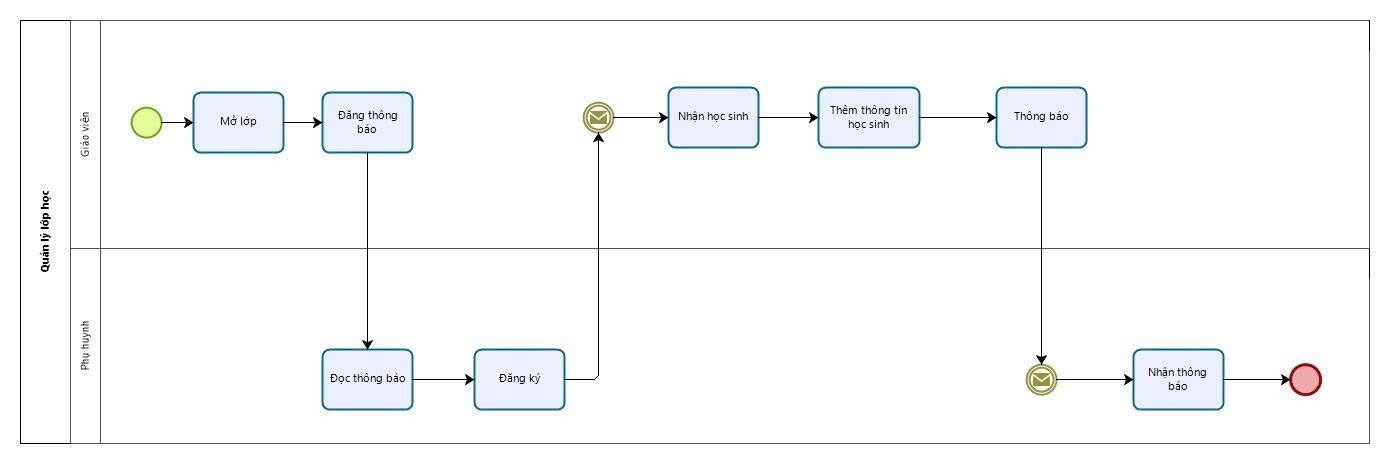
\includegraphics[width=1\textwidth]{picC1/QuanLyLopHocThem.jpg}
    \caption{Quy trình quản lý lớp học thêm}
\end{figure}

\begin{figure}[htbp]
    \centering
    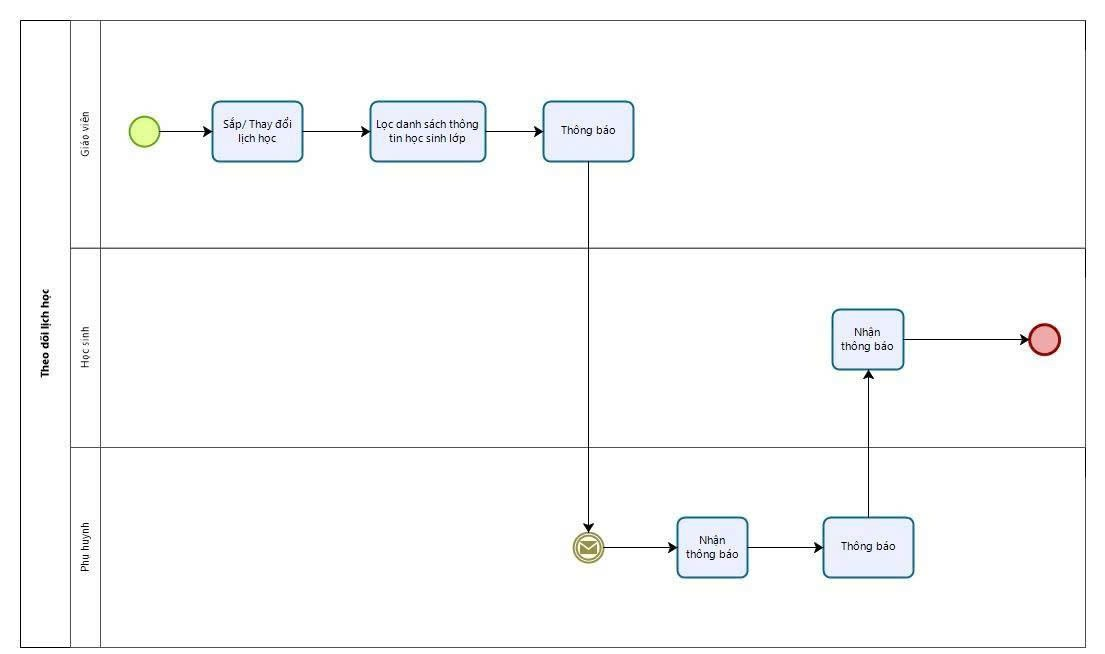
\includegraphics[width=1\textwidth]{picC1/TheoDoiLichHoc.jpg}
    \caption{Quy trình theo dõi lịch học}
\end{figure}

\begin{figure}[htbp]
    \centering
    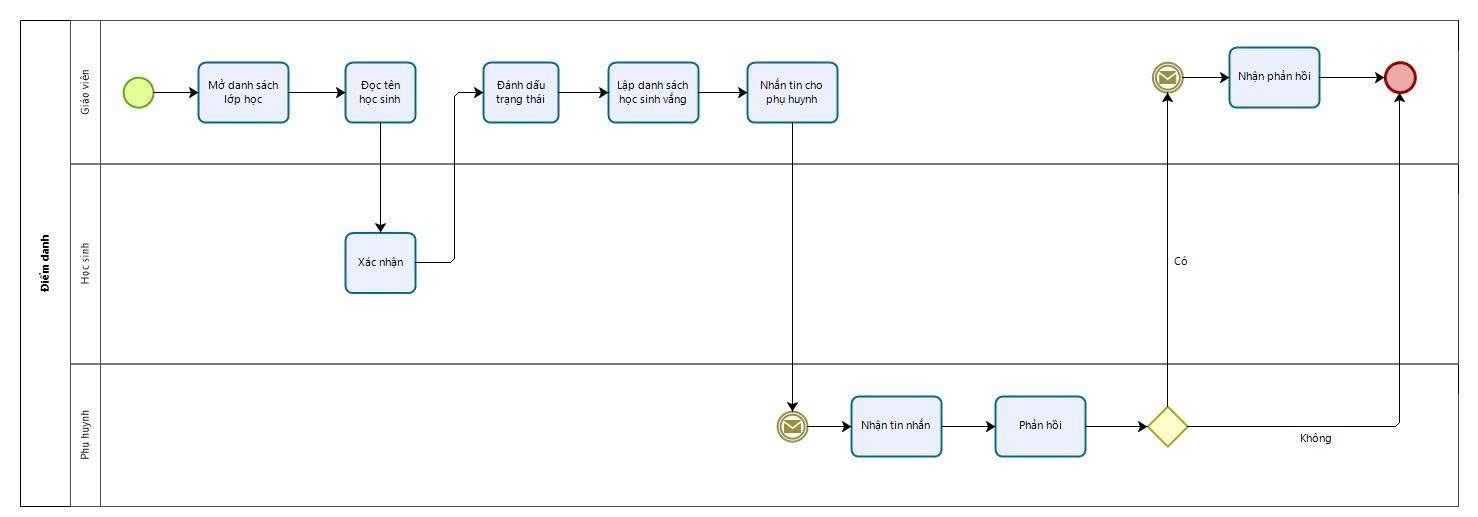
\includegraphics[width=1\textwidth]{picC1/DiemDanh.jpg}
    \caption{Quy trình điểm danh}
\end{figure}

\begin{figure}[htbp]
    \centering
    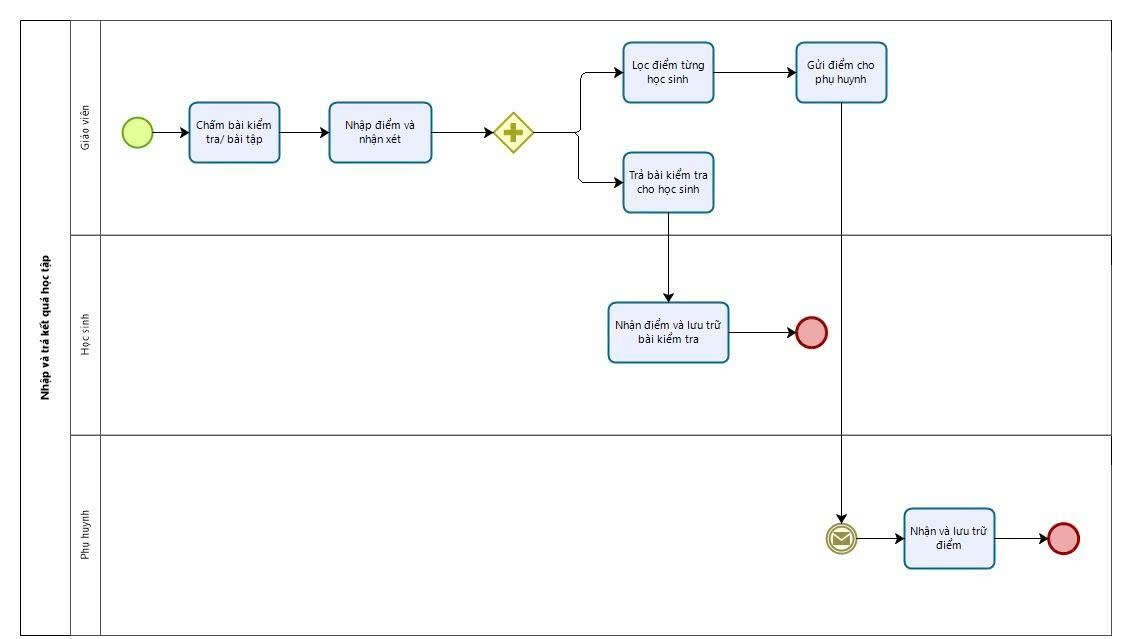
\includegraphics[width=1\textwidth]{picC1/NhapTraKQHT.jpg}
    \caption{Quy trình nhập/ trả kết quả học tập}
\end{figure}

\begin{figure}[htbp]
    \centering
    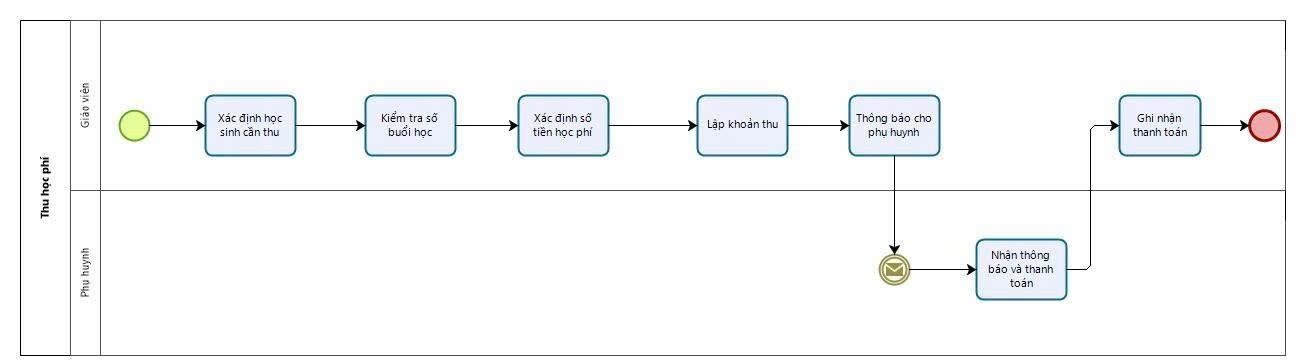
\includegraphics[width=1\textwidth]{picC1/ThuHocPhi.jpg}
    \caption{Quy trình thu học phí}
\end{figure}
\clearpage
\subsection{Biểu đồ phân cấp chức năng}
\section{Xây dựng kế hoạch dự án đơn giản}
\textit{<Xây dựng một bản kế hoạch thời gian, nhân sự và quản lý rủi ro đơn giản...>}